% --------------------------------------------------------
% Department of Information Engineering and Mathematics
% University of Siena, Italy
% Overleaf/LaTeX Template Created by Prof. Tommaso Addabbo
% --------------------------------------------------------

% use twoside option in case of double-sided print
\documentclass[12pt,a4paper,oneside]{report} 
\usepackage[utf8]{inputenc}

% customize your packages in the following file
% --------------------------------------------------------
% for PDF/A-1b pdf file - +++ DO NOT REMOVE THIS +++
% https://en.wikipedia.org/wiki/PDF/A
\PassOptionsToPackage{hidelinks}{hyperref}
\usepackage[a-1b]{pdfx}   

% --------------------------------------------------------
% set document margins and line spacing
\usepackage[top=45mm,bottom=35mm,inner=35mm,outer=25mm]{geometry}
\usepackage{setspace}
\setstretch{1.6}
% --------------------------------------------------------
% mathematical environment
\usepackage{amsmath}
\usepackage{amsfonts}
\usepackage{amssymb}
\usepackage{amsthm}
\usepackage{booktabs}
\usepackage{rotating}
\usepackage[nottoc,notlot,notlof]{tocbibind}
\usepackage{pdflscape}
\usepackage{diagbox}
\usepackage{multirow}
\usepackage{colortbl}
\usepackage{booktabs}
\usepackage{hhline}
%\usepackage{tablefootnote}
%\usepackage[nottoc,numbib]{tocbibind}
%\usepackage{natbib}

% --------------------------------------------------------
% figures, graphics, captions and table rows
\usepackage{graphicx}
\usepackage[justification=centering,font={small,singlespacing}]{caption}
\renewcommand{\arraystretch}{1.5}

% --------------------------------------------------------
% references, citations
\usepackage{cite} 

% --------------------------------------------------------
% headers and footers
\usepackage{fancyhdr}
\setlength{\headheight}{14.5pt}
\setlength{\footskip}{16mm} 

\usepackage{etoolbox}%

\usepackage{hyperref}

\newcommand{\makefootnotelist}[1]{%
    \parbox{0.8\textwidth} {%
        \footnotesize{%
            \renewcommand*{\do}[1]{##1\\}%
            \dolistcsloop{#1}}}}%
\renewcommand{\footnote}[1]{%
    \footnotemark{}%
    \def\listname{footlist\thepage}%
    \def\n{$^{\the\numexpr\value{footnote}}$}
    \ifcsdef{\listname}%
        {\listcseadd{\listname}{\n\ #1}}%
        {\csedef{\listname}{}%
        \listcseadd{\listname}{\n\ #1}}%
    \fancypagestyle{fancyfootnote}{%
        \fancyfoot[LO,RE]{\makefootnotelist{\listname}}%
        \fancyfoot[RO,LE]{\thepage}%
        \fancyfoot[C]{}%
    }\thispagestyle{fancyfootnote}}%

\fancypagestyle{default_page}{
\fancyhead[C]{}
\if@twoside%
    \fancyhead[LE,RO]{\sl CHAPTER \thechapter}
    \fancyhead[RE,LO]{}
\else
    \fancyhead[R]{\sl CHAPTER \thechapter}
    \fancyhead[L]{}
\fi
\fancyfoot[L,R]{}
\fancyfoot[C]{\small\thepage}
\renewcommand{\headrulewidth}{0.1mm}
}

\fancypagestyle{empty_page}{
\fancyhf{}
\renewcommand{\headrulewidth}{0pt}
\renewcommand{\footrulewidth}{0pt}
}

\fancypagestyle{final_stuff}{
\fancyhead[C]{}
\if@twoside%
    \fancyhead[LE,RO]{\sl \leftmark}
    \fancyhead[RE,LO]{}
\else
    \fancyhead[R]{\sl \leftmark}
    \fancyhead[L]{}
\fi
\fancyfoot[L,R]{}
\fancyfoot[C]{{\small\thepage}}
\renewcommand{\headrulewidth}{0.1mm}
}

% \usepackage{etoolbox}%

% \newcommand{\makefootnotelist}[1]{%
%     \ifcsdef{#1}%
%         {\parbox{0.8\textwidth} {%
%             \footnotesize{%
%             \renewcommand*{\do}[1]{#1\\}%
%             \dolistcsloop{#1}}%
%             %\renewcommand{#1}{}
%             }}%
%         {#1}%
%             }%

% \newcounter{mpFootnoteValueSaver}

% \newcommand{\fancyfootnote}[1]{%
%     \stepcounter{mpFootnoteValueSaver}%
%     \footnotemark[\value{mpFootnoteValueSaver}]{}%
%     \def\listname{footlist}%
%     \def\n{$^{\the\numexpr\value{mpFootnoteValueSaver}}$}
%     \ifcsdef{\listname}%
%         {}%
%         {\csedef{\listname}{}}%
%     \listcseadd{\listname}{\n\ #1}}
    
% \renewcommand{\footnote}[1]{%
%     \fancyfootnote{#1}}

\makeatletter
\def\emptypage@emptypage{%
    \thispagestyle{empty}
    % \hbox{}%
    \vspace*{\fill}
    \begin{center}
    {\footnotesize This page intentionally left blank.}
    \end{center}
    \vspace{\fill}
    \newpage%    
}%
\def\cleardoublepage{%
        \clearpage%
        \if@twoside%
            \ifodd\c@page%
                % do nothing
            \else%
                \emptypage@emptypage%
                
            \fi%
        \fi%
    }%
\makeatother


% --------------------------------------------------------
% handle links and urls
\usepackage{url}

% --------------------------------------------------------
% code listing
\usepackage{listings}




% ========================================================
% ========================================================
\begin{document}

% ========================================================
% ========================================================

\pagestyle{empty_page}


% --------------------------------------------------------
% cover page
\newgeometry{top=12mm,bottom=15mm,inner=25mm,outer=25mm}
\begin{titlepage}
\begin{spacing}{1.4}
%
\begin{figure}[ht]
\centering

\includegraphics[height=100mm]{FIGURES/logoConcordia.pdf}
\end{figure}
%
\begin{center}
{\scshape \Large
Department of \\ Computer Science and Software Engineering 
}

\vspace{5mm}

\rule{100mm}{0.1mm}
\rule[5mm]{100mm}{0.4mm}

{\large 
Ph.D. Program \\ 
{Computer Science}
}

\vspace{12mm}

\begin{spacing}{2.0}
{\huge \bf ENCS-8501 Comprehensive Exam}
\end{spacing}

\end{center}

\vspace{8mm}
\noindent
\begin{minipage}[t]{0.5\textwidth}
\bf Supervisor:\\
Dr. Sandra Céspedes\\
 
Evaluation committee:\\
Prof. Yann-Gael Gueheneuc, CSSE \\
Prof. Essam Mansour, CSSE\\
Prof. Chadi Assi, CIISE\\

\end{minipage}
\hfill
\begin{minipage}[t]{0.5\textwidth}\raggedleft
\bf Candidate:\\
Alexis Yáñez\\
ID. 40244341
\end{minipage}

\vfill

\begin{center}
\large Fall 2023 Term
\end{center}

\end{spacing}


\end{titlepage}
\restoregeometry

\cleardoublepage 
\setcounter{page}{1}

% --------------------------------------------------------
% table of contents
\tableofcontents
\cleardoublepage
\pagestyle{default_page}


% --------------------------------------------------------
% input your chapters here

%---------------------------------------------------------
\chapter{Introduction}
%---------------------------------------------------------

In recent years, the deployment of 5G/Beyond 5G and C-V2X (Cellular Vehicle-to-Everything) networks has paved the way for deploying real-time vehicular safety applications \cite{ul2019green}. Thanks to the reduction of delays and the appearance of different architectures, information can be easily and safely exchanged between different actors on the traffic routes \cite{tudzarov2011functional}. C-V2X technology allows different modes of communication to connect cars and Vulnerable Road Users (VRU). 

%In fact, over C-V2X network, it is possible to dispense with equipment dedicated to establishing vehicle networks (as was formerly used in the IEEE 802.11p protocol), allowing smartphone’s use to constitute the network structure. 
In fact, over the C-V2X network, it is possible to establish communication between devices such as smartphones enabled to work with this network. This way, vulnerable users such as pedestrians, cyclists, and others can participate in the vehicular network. The inclusion of VRU was not straightforward over the IEEE 802.11p standard since network participants needed dedicated equipment for exchanging messages over the wireless network.


The usage of C-V2X through smartphones or other VRU devices (e.g., 5G-enabled smart helmets) also poses a series of challenges to consider. One of the main challenges is managing congestion over the communications network, as the number of devices connected to the network may increase significantly. The density of devices in crowded vehicular scenarios represents a challenge to the operation of the vehicular network. Recent proposals of architectures and device groupings tackle the device crowding problems, including over-signaling and networks collapsing \cite{hakeem20205g}.

This is a report of the literature review conducted on the topic of Collective Perception Service (CPS) and its relationship with VRU detection.%  a topic directly related to the doctoral thesis proposal.  
For this purpose, we reviewed recent articles published in journals and conferences of significant impact and recognized by the international scientific community. The remainder of this document is organized as follows: Chapter 2 presents the study of the literature agreed upon with the Advisor. Chapter 3 discusses and critically analyzes the possible research gaps that have not been covered or are posed as future challenges. Finally, Chapter 4 provides the work plan for the development of the doctoral thesis. 
\cleardoublepage % opens next new chapters in right pages for two-sided printing

%    El capítulo de revisión necesita una mejor estructura. Hasta donde vi tienes un conjunto de papers que discuten \textbf{Sistemas de detección} de VRU. Otro tema puede ser directamente el de\textbf{ Collective Perception Systems (más formalmente como está definido por la ETSI).} Necesito que pienses en subsecciones.
% Una vez tengas las subsecciones, para cada paper revisado asegúrte de identificar: qué proponen, cómo lo hicieron, qué resultados lograron, fortalezas y desventajas. Las frases que puedes usar son: In [X] the authors propose bla bla. In the methodology, they used bla bla and modeled bla bla, etc. The results showed that bla bla. The streghts of this work are bla bla; on the other hand, the weakness of this work are bla bla.  Trata de mantener mas o menos la misma estructura cada vez que presentes un paper nuevo
%Mueve la tabla resumen de todos los trabajos a la sección de discusión. Trata de hacer un compilado de las debilidades más remarcadas (o las que más se repiten) en los trabajaos revisados. En future work sería bueno eferencias al menos uno o dos trabajos que propongan el tema de clustering, como un antecedente (puede ser uno de los ya revisados)
%Simplifica el workplan a algo parecido a como lo presentó Raydel y donde se pueda ver lo que se YA se hizo en el período pasado (un año antes)

%---------------------------------------------------------
\chapter{Literature Review}
%---------------------------------------------------------
Nowadays, we observe a substantial integration of new wireless access technologies to support the deployment of Intelligent Transportation Systems (ITS) Applications. New proposals and standardization have succeeded in expanding the use cases and performance of information services related to intelligent and efficient transportation management. In fact, wireless access networks have been considered a critical factor in realizing ITS applications \cite{5GAA}. 

One advantage of using wireless networks in the traffic context is that the information collected by both motor vehicles and infrastructure can be shared with the different users of the traffic network. This corresponds to the information collected individually by sensors in modern vehicles and equipment installed in the infrastructure of the traffic roads. Collection and sharing of information from the environment---through sensors or other techniques---involve new challenges that have been addressed mainly from a sensor fusion approach, where the main purpose is to share obstacle detection by vehicles with other vehicles on their neighborhood. Accordingly, the concept of Collective Perception has been defined by ETSI \cite{ETSI}, where one of the most important challenges is dealing with communication channel overload and redundant information reported in the vehicular context. 

One of the aspects to be addressed by the collective perception corresponds to the detection of Vulnerable Road Users (VRU) such as pedestrians, cyclists, electric scooter riders, and motorcyclists, among others. VRU detection is an important feature in assisted and autonomous driving. The use of information collectively generated from VRU detection systems is a topic under research and currently under standardization. 
%---------------------------------------------------------
\section{Collective Perception Service}
%---------------------------------------------------------
The Collective Perception Service is a concept defined by ETSI in \cite{ETSI} as follows:
\begin{quote}
\textit{Concept of sharing the perceived environment of a station based on perception sensors}
\end{quote}
A station corresponds to an Intelligent Transport Systems-Station (ITS-S) that could be present in the infrastructure, vehicles, or people.
Besides the concept, the report defines services and uses cases, like Generation Rules for Collective Perception Messages (CPM), which differ from the Cooperative Awareness Messages (CAM). CPM are messages intended to share the perceived environment, and CAM are messages intended to share the dynamic state of each vehicle \cite{ETSI2}.

One of the main access technologies to support the Collective Perception Service in ITS is 5G-CV2X. The authors in \cite{hakeem20205g} performed an extensive study of the 3GPP releases 14 and 16 regarding the implementation of 5G-V2X. The authors provided precise details on the technologies involved, challenges, features, requirements, and designs. Something to highlight in their study corresponds to the analysis of the use cases, where they specifically mentioned the \textit{Use Case 3 (UCC3): Cooperative safety}, defined as follows:

\begin{quote}
``Use Case 3 (UCC3): is mainly concerned with protecting Vulnerable Road Users (VRUs). This can be done by detecting the presence of VRUs using a local sensor or camera or radar or using a positioning system, or using the communication system. Another way to detect the presence of VRUs is by using their cellular phone information if the VRU holds a smartphone or a cellular communication device."
\end{quote}

According to Use Case 3 discussed in \cite{hakeem20205g}, smartphones are proposed to detect VRU. However, the authors did not include the design and evaluation of new ways to warn about the presence of VRU using the communications network using device-to-device communications, discarding how much progress could be made in this area, such as grouping VRU to establish resource allocation for safety message exchanges. In the emerging needs of this case, they remarked on the inclusion of new sensors for the passive recognition of VRUs, discarding the active role of these users on the communications network.

In \cite{Ghorai2022}, the authors describe extensive research on the state estimation and motion prediction of vehicles and vulnerable road users for cooperative autonomous driving. In the study, the authors detailed several proposals for VRU and vehicle detection in transit roads, considering this task as a primary one in the development of environment discovery capabilities of autonomous vehicles. In the first instance, the study describes the different sensors, methods, and techniques for detecting VRUs or animals. About the detection of cyclists and pedestrians, the study mentions the following:

\begin{quote}
``More research is still needed in this area (Pedestrian, Cyclist, and Vehicle Detection) since the mAP (Mean Average Precision) of the current methods, especially when it comes to pedestrians and cyclists that are more vulnerable and frequently disobey traffic laws, is far lower than 90\%".
\end{quote}

Nevertheless, the study makes little mention of the possibility of pedestrians and cyclists being able to participate in the communication network; the focus of the study in question is strongly related to the different sensors deployed in the vehicles and other methods to exploit them.

%Thanks to the two works mentioned above \cite{hakeem20205g,Ghorai2022} it is possible to access many proposals that are highly related to the object of study that supports this report. Both works allow us to understand many technologies, methods, and techniques for VRU detection and how different challenges associated with implementing and developing these systems originated.

\section{Detection of Non-Connected Road Users}

In \cite{Rondinone2018}, the authors propose a system architecture that, based on collaborative information between vehicles and the infrastructure, can deploy safety applications. The architecture proposed in the work detailed above is shown in Fig \ref{fig:Rond}. This work is strongly related to Cooperative Autonomous Vehicles (CAV). In the system, VRU are considered as objects, or non-cooperative users, to be included in the information shared between vehicles. The work is framed under the ETSI-ITS G5 standardization and it aims at describing the V2X solutions adopted by the EU funded project H2020 MAVEN (Managing Automated Vehicles Enhances Network)\footnote{http://www.maven-its.eu/}. The authors in \cite{Rondinone2018} discard the active role of VRUs on the vehicular network context. 

\begin{figure}[ht!]
    \centering
    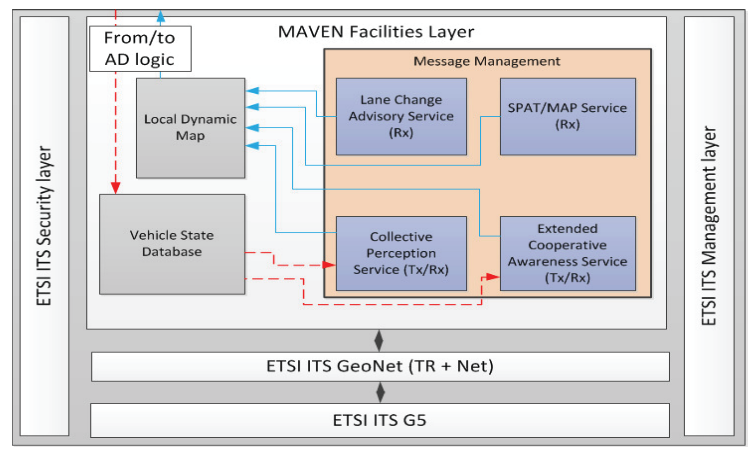
\includegraphics[width=10cm]{FIGURES/Fig2.png}
    \caption{MAVEN CAV communication architecture. Source: \cite{Rondinone2018}}
    \label{fig:Rond}
\end{figure}

In \cite{DaSilva2019}, the authors focused on the fusion of information from other vehicles, connected through IEEE 802.11p, with which VRU detection is performed. They did not consider connectivity for VRU. Furthermore, the authors describe a flexible end-to-end system simulator that can evaluate cooperative mapping strategies in complex road driving environments. As shown in Figure \ref{fig:DaS}, the proposed system requires an infrastructure where the information about environment maps are sent to the station. Once the base station collects the maps from every vehicle in the surrounding area, it runs the detection process.

\begin{figure}[ht!]
    \centering
    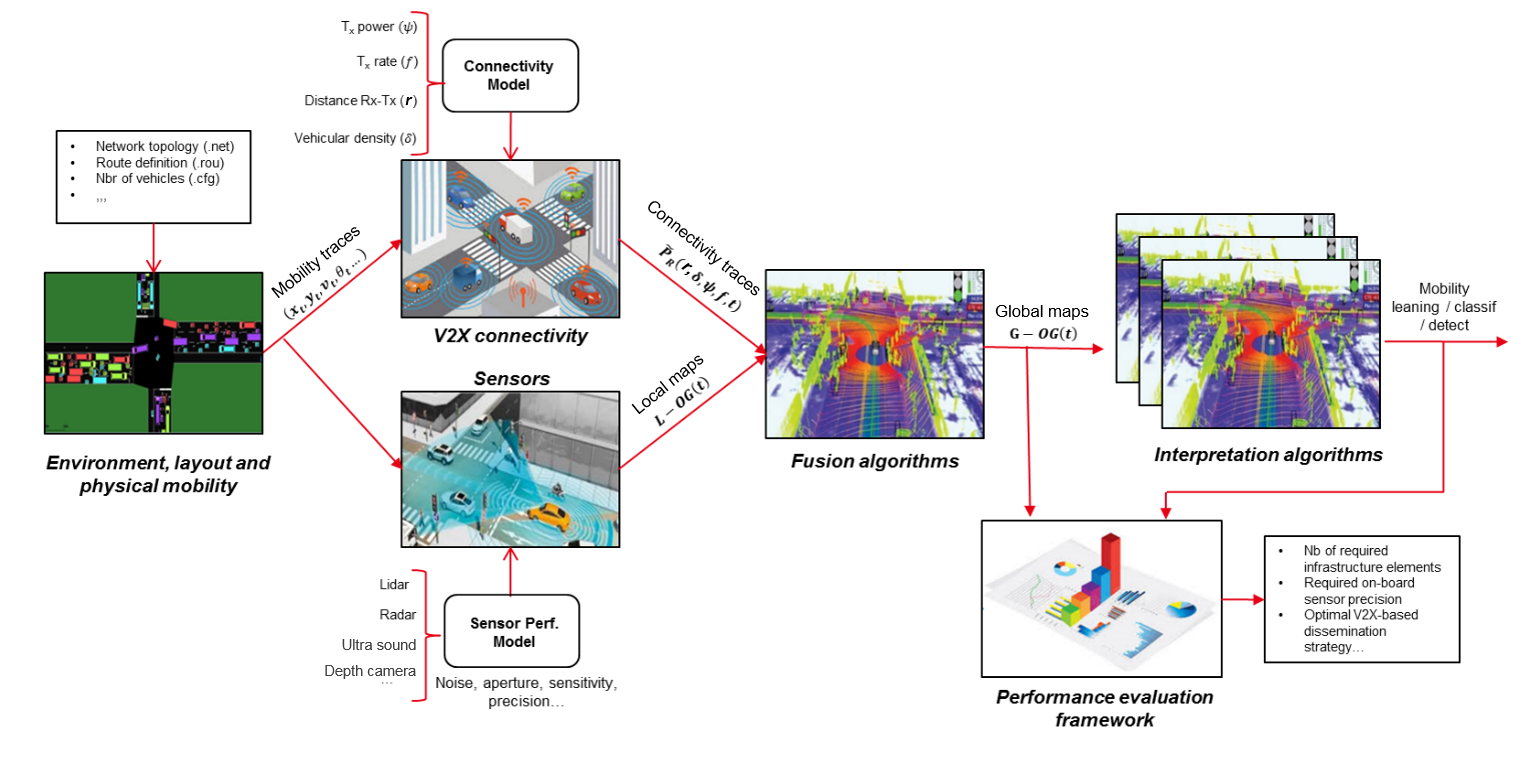
\includegraphics[width=15cm]{FIGURES/Figura5.png}
    \caption{Dataflow for the proposed system Source: \cite{DaSilva2019}}
    \label{fig:DaS}
\end{figure}

Subsequently, in \cite{Tsukada2020}, the authors proposed AutoC2X, a system that enables cooperative perception using OpenC2X for autonomous vehicles based on Autoware. The proposed system (see Figure \ref{fig:Tsu}) was initially tested in software implementation contexts and then field-tested with real equipment. This proposal's full development focuses on providing better environmental information to autonomous vehicles. The results showed that the system can reduce the delivery times of collective perception messages up to $100 [ms]$ in the worst-case scenario. They considered VRU as passive since they are categorized as obstacles. The experiments involved infrastructure, such as roadside units, to obtain environmental information reported by autonomous vehicles. 

\begin{figure}[ht!]
    \centering
    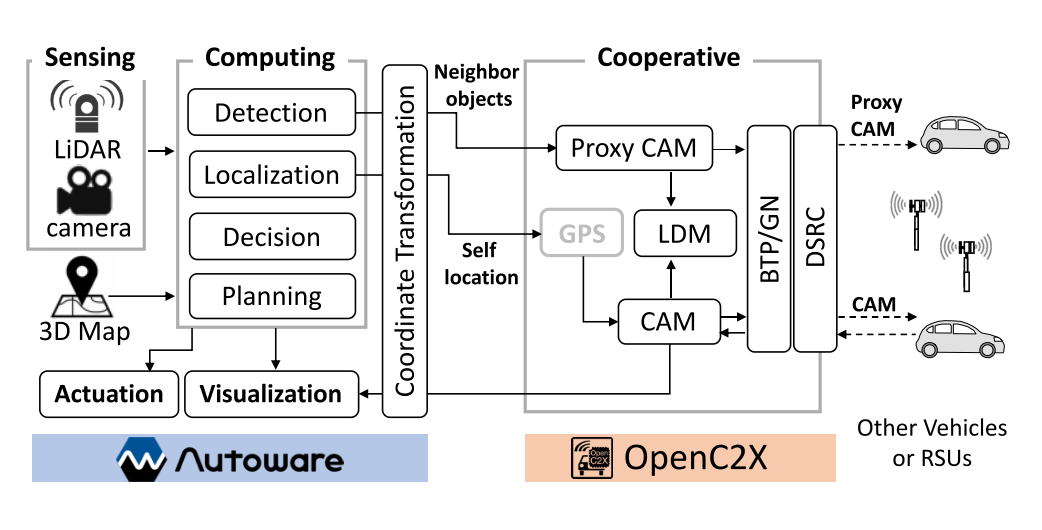
\includegraphics[width=10cm]{FIGURES/Fig7.png}
    \caption{Architecture for the proposed system. Source: \cite{Tsukada2020}}
    \label{fig:Tsu}
\end{figure}

In \cite{Schiegg2021}, the authors presented a system for generating collective perception messages based on the implementation of sensor-equipped infrastructure for VRU protection. This covers areas with blind spots where vehicle sensors have poor performance. The authors presented the design of their proposal (see Figure \ref{fig:Sch}) in addition to performing empirical evaluations with a real experiment and with simulations. The results showed that the proposed system works properly under low density scenario. However under the large-scale assessment, the authors identified a lack in the delivery of information about the collective perception messages due to highly congested scenarios; to address the latter, the authors proposed to give priority to the link for Infrastructure to Vehicle (I2V) rather than for Vehicle to Vehicle (V2V) in what is known as resource allocation.

\begin{figure}[ht!]
    \centering
    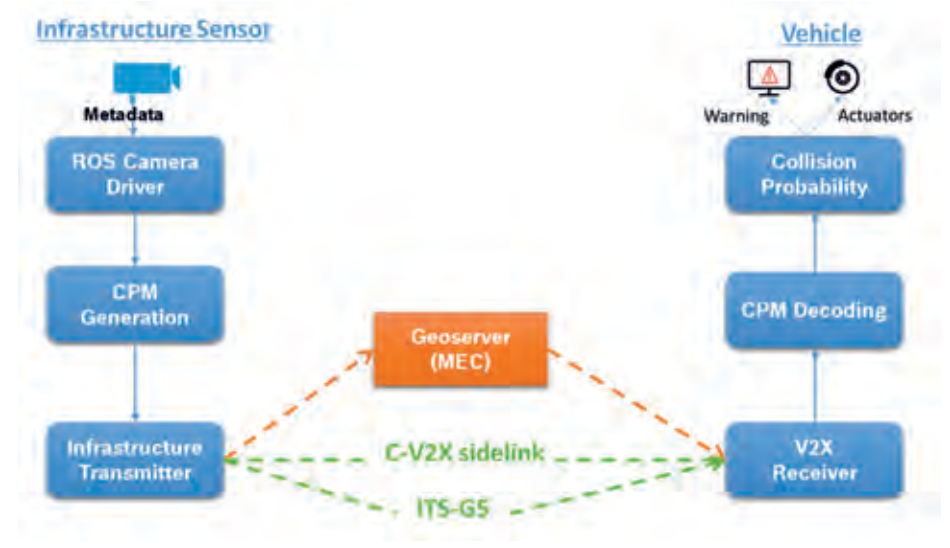
\includegraphics[width=10cm]{FIGURES/Fig9.png}
    \caption{System architecture of the VRU protection use case. Source: \cite{Schiegg2021}}
    \label{fig:Sch}
\end{figure}

In \cite{Jan2021}, the main contribution from the authors is the introduction of a tool for the generation of virtual pedestrians that realistically avoid obstacles, providing a platform to accurately and efficiently test autonomous vehicles in pedestrian areas. In this way, they provided a tool for to emulate a scenario where an autonomous vehicle enters an environment with moving pedestrians. This work considered not only individuals but also studied cases of interaction with groups of people moving in pedestrian zones. The latter is relevant because it is one of the few articles that refer to the detection of individuals and groups of people. Figure \ref{fig:Jan} shows a view of the simulation tool where pedestrians and an autonomous vehicle interact. 

\begin{figure}[ht!]
    \centering
    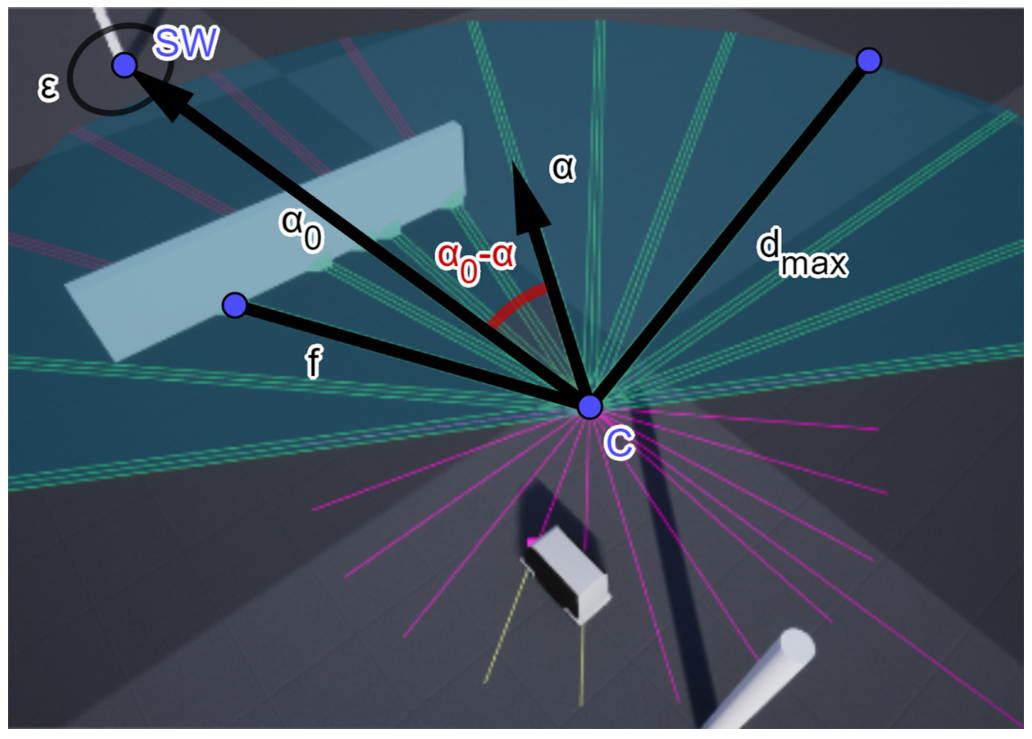
\includegraphics[width=10cm]{FIGURES/Fig11.png}
    \caption{Simulation view of virtual pedestrian c in the vehicle's vicinity and an obstacle. Source: \cite{Jan2021}}
    \label{fig:Jan}
\end{figure}

\section{Fusion Sensor and Connected VRU}

In \cite{Merdrignac2017}, the authors propose a VRU detection system, where VRU can connect with motorized vehicles using IEEE 802.11g. The system exploits the information coming from sensors deployed in each car and employs techniques for the fusion of the information received by each vehicle. The study shows that an ideal fusion between perception and Vehicle to Pedestrian (V2P) communication should benefit from both systems. Figure \ref{fig:Merd} shows the overall cooperative protection system description and a flow chart of the fusion between perception and V2P communication. Furthermore, the authors considered when there is line-of-sight (LOS) and non-line-of-sight (NLOS) at the moment the detection is performed. Additionally, the article presents the evaluations of an empirical experiment and contrast it with the theoretical models. Note that this work did not consider any scheme or assumption about the grouping of VRUs or motor vehicles.

\begin{figure}[ht]
    \centering
    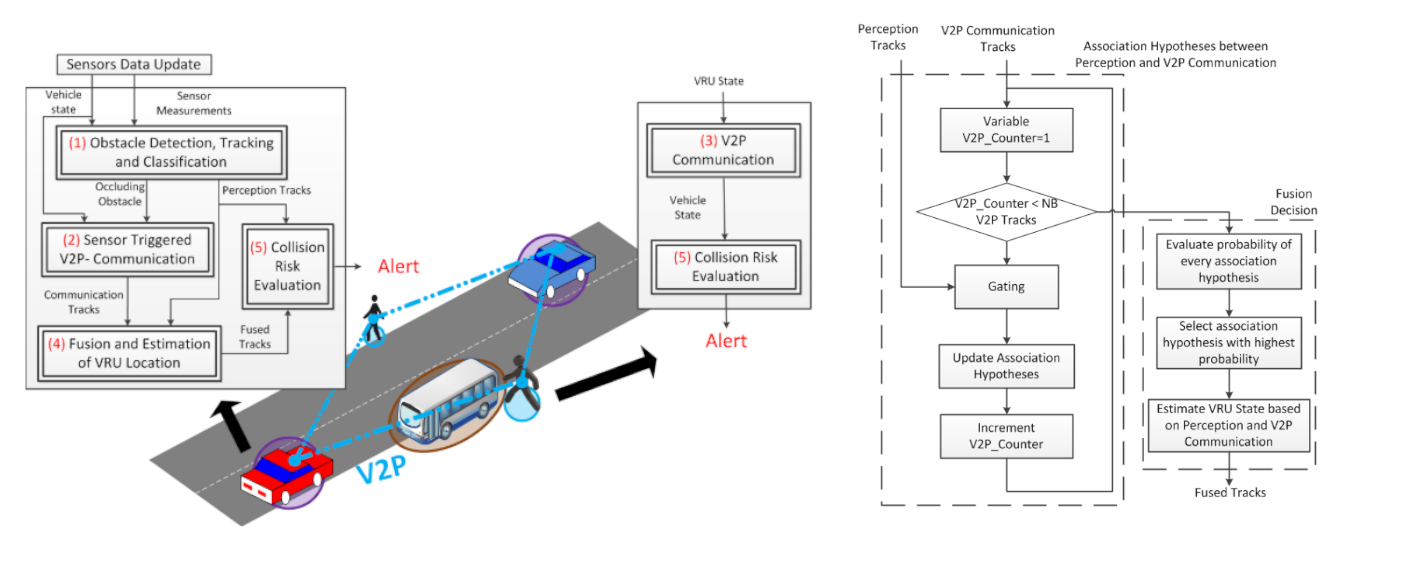
\includegraphics[width=16cm]{FIGURES/Fig1.png}
    \caption{Cooperative protection system description (left) and flow chart of fusion between perception and V2P communication (right). Source: \cite{Merdrignac2017}}
    \label{fig:Merd}
\end{figure}


In \cite{Reitberger2018}, the authors presented an approach to the cooperative tracking of cyclists using smart devices and infrastructure-based sensors. Although the study did not mention a specific technology for the exchange of information between the infrastructure and cyclists, the authors referred to the use of an ad-hoc network for the reception of variables associated with the cyclist's movement (e.g., the speed) for the infrastructure to track it (see Figure \ref{fig:Rei}). This work is mainly oriented to the theoretical analysis of how to track VRU from the infrastructure. In the experiment, the intersection is equipped with a stereo camera, also they assume an ideal communication medium with negligible
delay. However, they proposed using a more realistic communication network model in their future work. The work does not report what is intended to be done with the VRU tracking: if it will update a database or will transmit tracking information to the vehicles in the communications network.\begin{figure}[ht!]
    \centering
    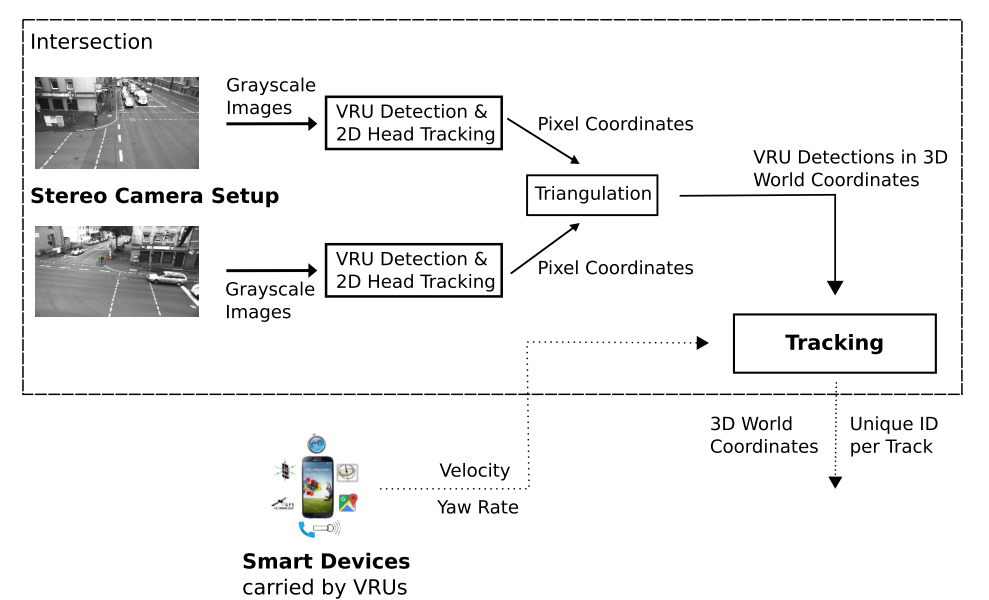
\includegraphics[width=12cm]{FIGURES/Fig3.png}
    \caption{VRU tracking based on infrastructure and smart devices. Source: \cite{Reitberger2018}}
    \label{fig:Rei}
\end{figure}

Continuing with the literature review, in \cite{Sewalkar2019}, 
the authors first presented a literature study related to the integration of VRU in the context of wireless communication network development and the technologies used for this purpose. Then, they evaluated via simulations the implementation of rules for the generation of messages from VRU, taking into consideration their dynamics. Therefore, they considered active VRU. For evaluating their proposal, they used a simulation of an intersection as the one shown in Figure \ref{fig:Sew}. Within the discussion of their results, they highlighted the importance of VRU's active role in communications. In addition, they showed---as it has been supported in other works---that the use of VRU devices would significantly increase the load on the communication network. The authors mentioned some of the efforts to deal with the congestion problem, among which are the creation of reception-only modes, contextual transmission, and VRU clustering.

\begin{figure}[ht!]
    \centering
    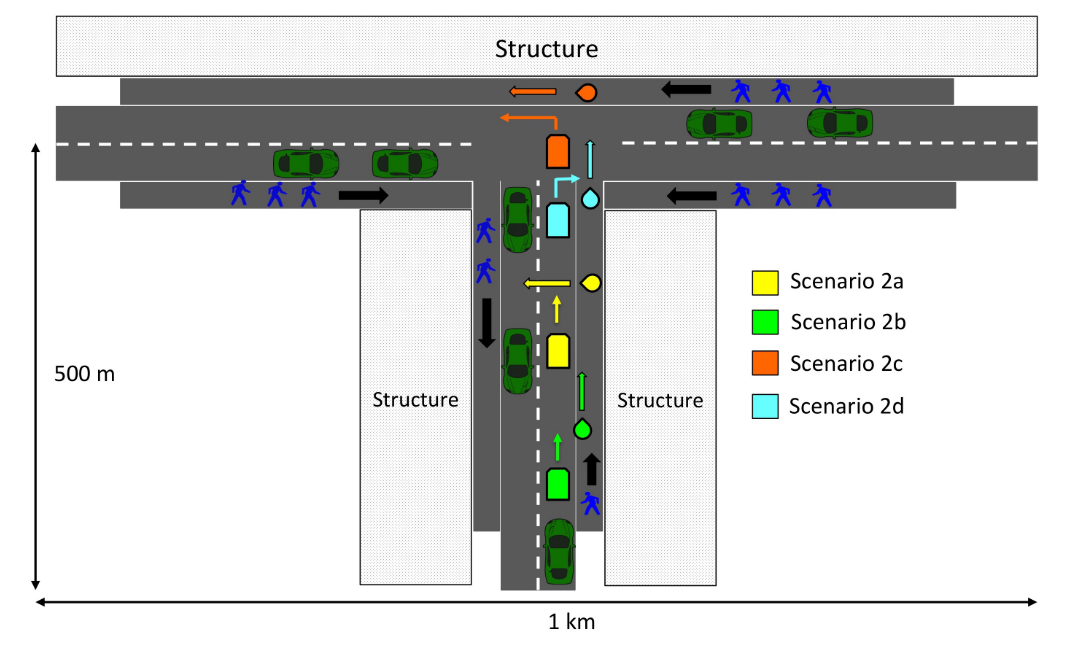
\includegraphics[width=10cm]{FIGURES/Fig6.png}
    \caption{Simulation scenario, source:\cite{Sewalkar2019}}
    \label{fig:Sew}
\end{figure}

In \cite{Emara2020}, the authors used the Age-of-Information (AoI) metric and evaluated a system where VRU send messages over the C-V2X scheme, i.e., from their devices to a base station (see Figure \ref{fig:Ema}). With this, they evaluated the performance of metrics such as packet inter-arrival time for detecting these users by motor vehicles. Additionally, they established a considerable improvement over the metrics discussed above by using a Multiple-access Edge Computing MEC architecture. The performance evaluation has been done using analytical models. 

\begin{figure}[ht!]
    \centering
    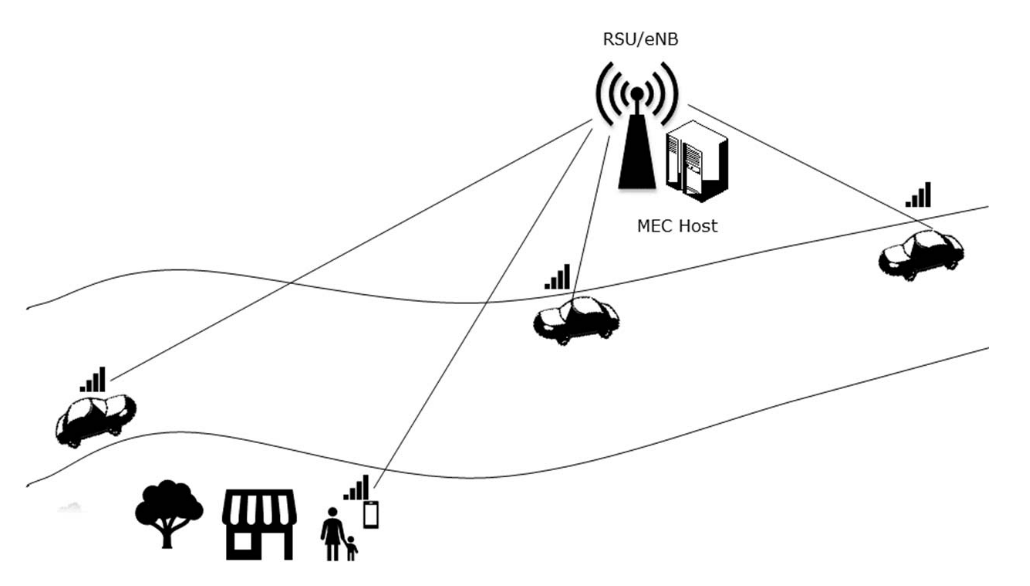
\includegraphics[width=10cm]{FIGURES/Fig8.png}
    \caption{Evaluation scenario. Source:\cite{Emara2020}}
    \label{fig:Ema}
\end{figure}

Authors in \cite{Militaru2021} proposed an interactive traffic application based on robust connectivity of all traffic participants and intelligent infrastructure. As shown in Figure \ref{fig:Mil}, the proposed application is based on an established architecture where different options for VRU and vehicle connection exploiting WiFi, BLE, and CV2X networks are considered. The application seeks to alert the presence of VRUs on the roads using sensors and cooperative perception messages. However, no evaluation of the proposed application is evidenced by simulations or experimental tests.


\begin{figure}[ht!]
    \centering
    \includegraphics[width=13cm]{FIGURES/Fig13.png}
    \caption{Interface Application usage in a traffic scenario and the proposed architectures. Source: \cite{Militaru2021}}
    \label{fig:Mil}
\end{figure}


\section{Generation Rules Techniques and Redundancy Mitigation}

In \cite{Thandavarayan2019}, the authors discussed about the implementation of cooperative perception message generation rules, which aim to improve the information sharing about obstacle discovery with vehicles in the neighborhood. They performed an analysis using traffic and communication network simulations, where they evidenced differences when establishing dynamic message generation policies over time in contrast to fixed frequency message generation policies. Authors also evaluated the impact of these rules on high and low denial of service scenarios. Moreover, they established a metric to measure the collective awareness of discovered objects and evaluated the performance of the communication network using dynamic and static rules approaches. Figure \ref{fig:Than} show the different levels of awareness in each evaluation case. The results reported significant differences when there is a greater distance between the obstacles and the vehicle that discovers them. At the same time, it is evident how the use of these rules directly impacts the performance statistics of the communications network, e.g., the packet delivery ratio (PDR). In this work, a passive role is considered from the VRUs as they do not participate in the exchange of cooperative perception messages. 
\begin{figure}[ht!]
    \centering
    \includegraphics[width=15cm]{FIGURES/Fig4.png}
    \caption{Object Awareness Ratio as a function of the distance between the detected object and the vehicle receiving the CPM (Left), PDR (Packet Delivery Ratio) as a function of the distance between transmitter and receiver (Right). Source: \cite{Thandavarayan2019}}
    \label{fig:Than}
\end{figure}

In much the same way as the previous article, in \cite{Garlichs2019}, the authors contribute to the invention of a set of generation rules for the Collective Perception Service, which seek to handle the trade-off between two important aspects in the performance of vehicular networks: 1) provide quality of service to receiving Intelligent Transport System stations, in terms of the number of known objects and the update frequency per unique object known; and 2) reduce the generated network load on the employed radio channel.

Unlike the authors in \cite{Thandavarayan2019}, in \cite{Garlichs2019} they established more complex generation rules that consider the following characteristics of the detected object: novelty, distance, speed, and age. In addition, they included in their system the segmentation of cooperative messages to reduce the radio channel load and thus improve the statistics of the communication network. 

In \cite{Willecke2021}, the authors analyzed the inclusion rules of person-like objects in a large-scale simulation study, demonstrating that exchanging cooperation messages can significantly improve people's awareness with little additional use of channel resources. For adding a new person or VRU to the cooperative perception messages, they use the scheme shown in Figure \ref{fig:will}, which is taken from another publication. The main contribution of this work lies in the large-scale simulation of the evaluation scenario. In the paper, they concluded that using the rules improves the congestion conditions of the channel when the number of obstacles to be discovered increases. 

\begin{figure}[ht!]
    \centering
    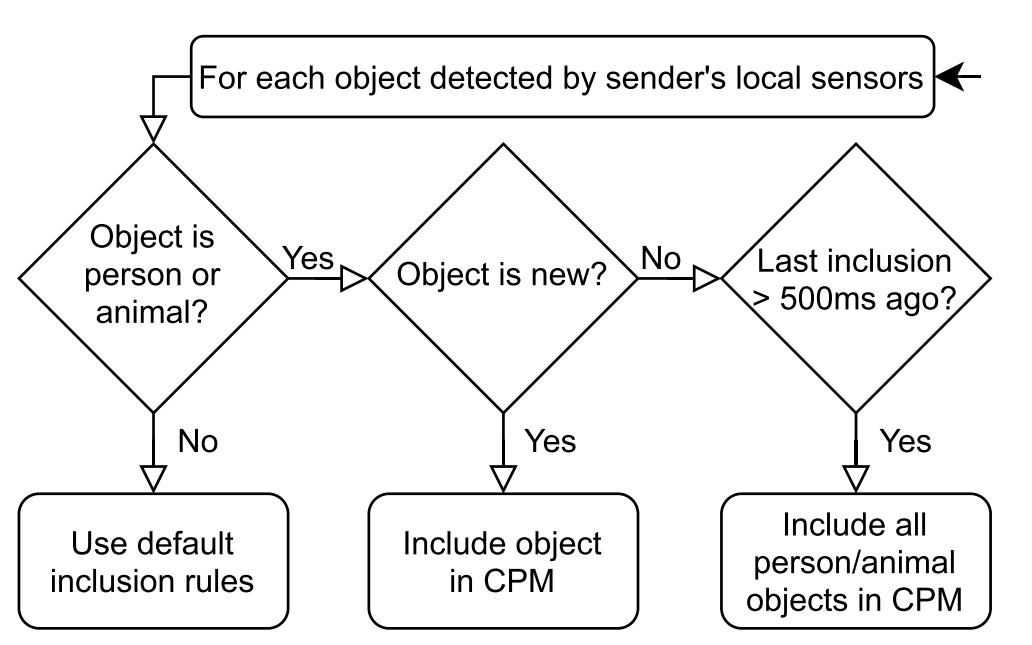
\includegraphics[width=10cm]{FIGURES/Fig10.png}
    \caption{Inclusion rules for objects of type person or animal currently defined in TR 103 562 (ITS standardization) Source: \cite{Willecke2021}}
    \label{fig:Will}
\end{figure}

In \cite{Delooz2022}, the authors analyzed, evaluated and compared rules for the inclusion of new obstacles recognized by sensors. These rules focused on mitigating redundant information within the communication network in the vehicular context due to the reporting of the same object by two or more vehicles or infrastructure in its vicinity. From the analysis of simulations, the authors implemented the rules of mitigation of redundant information by taking four filters through which the data should be checked (see Figure \ref{fig:Del}). The results showed that implementing these rules positively impacts the communication network, decreasing the load on the communication network without compromising the vehicle's awareness of obstacles or VRUs. The authors recognized that adjusting the rule parameters according to the load state of the communication network will increase its performance in terms of collective awareness and efficient use of network resources.  

\begin{figure}[ht!]
    \centering
    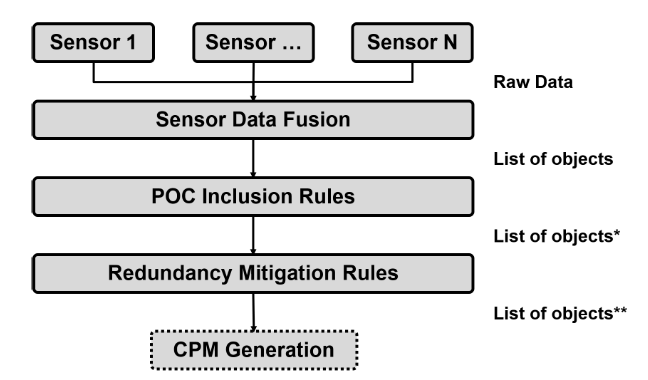
\includegraphics[width=10cm]{FIGURES/Fig12.png}
    \caption{dataflow for the proposed system Source: \cite{Delooz2022}}
    \label{fig:Del}
\end{figure}

%\newgeometry{top=1.7cm}


\cleardoublepage % opens next new chapters in right pages for two-sided printing

%---------------------------------------------------------
\chapter{Discussion and Future Work}
%---------------------------------------------------------
After the literature review carried out in this report, it can be evidenced that considering VRU is important because the safety of the road is increased, especially in automated systems such as assisted and autonomous driving.on the other hand, less than half of the articles studied consider an active role for VRUs. Where active role is assumed, VRU awareness increase significantly.

According to the study, the research gaps founded are describe following:

\begin{itemize}
    \item The lack of a realistic simulation scenario, in terms of the number of devices that can be had when considering active VRU.    
    \item The lack of a dynamic use in the architecture and resources of the network, in relation to facing different contexts of density and mobility.    
    \item The lack of grouping management schemes in detection systems for autonomous or motorized vehicles and VRU. 
    \item There is no evidence about how the grouping of VRU (if they take an active role) could benefit the use of the radio channel established for information exchange. 
    \item The lack of consensus on which architecture network to use for VRU's detection.
\end{itemize}


In our opinion there is a high dependence between this gaps and the standardization processes by institutions such as IEEE, ETSI, and 3GPP, among others; and how these processes can address the development of these gaps in terms of which aspects to develop are priorities. 

In the future work, we could consider the inclusion of different rules already established in the state-of-the-art and how these can be affected when we work with clusters and intelligent grouping of VRU 


\section{Comparison of Articles}

A summary of each of the works studied is presented in Table \ref{CollectiveTable}, detailing the technology they propose, the type of evaluation and experimentation they use if they consider groups within the context, the architecture they exploit and the role played by VRU within their scheme. 

It can be evidenced that six out of fourteen papers consider an active role for VRU, representing that the inclusion of VRU in the context of wireless communication networks in the vehicular context is incipient. 

On the other hand, the architectures used for both VRU detection and dissemination of VRU detection are different according to the approach given by their authors, making evident a lack of consensus on which architecture to use for this goal. 


\begin{center}
\begin{table}[ht!]
\caption{Comparison of all articles selected}
\label{CollectiveTable}
\resizebox{5.9in}{!}{%
\begin{tabular}{@{}lllllllr@{}}
\toprule
Article                 & Sensors                                                                                    & Communications                                               & \begin{tabular}[c]{@{}l@{}}Individual or \\ group approach\end{tabular}                & \begin{tabular}[c]{@{}l@{}}Experimental \\ Setting\end{tabular}              & Architecture & VRU     & \multicolumn{1}{l}{Year} \\ \midrule
\hline
Merdrignac, P. et al \cite{Merdrignac2017} %Merdrignac, P. et al
& \begin{tabular}[c]{@{}l@{}}Laser Based \\ on Cars\end{tabular}                             & IEEE 802.11g                                                 & \begin{tabular}[c]{@{}l@{}}Individual VRU \\ Cooperative \\ Vehicles\end{tabular}      & \begin{tabular}[c]{@{}l@{}}Theoretical and \\ Empirical results\end{tabular} & V2P          & Active  & 2017                     \\
\hline
Rondinone, M. et al \cite{Rondinone2018} %Rondinone, M. et al
& \begin{tabular}[c]{@{}l@{}}Vehicle Sensors \\ on board\end{tabular}                        & ETSI ITS G5                                                  & \begin{tabular}[c]{@{}l@{}}Cooperative \\ Vehicular \\ Group\\ Formations\end{tabular} & -                                                                            & V2I - V2V    & Passive & 2018                     \\
\hline
Reitberger, G. et al \cite{Reitberger2018} %Reitberger, G. et al 
& \begin{tabular}[c]{@{}l@{}}Stereo Camera \\ in Intersection \\ Infrastructure\end{tabular} & Ad-hoc network                                               & Individual VRU                                                                         & Theoretical                                                           & P2I          & Active  & 2018                     \\
\hline
Thandavarayan, G. et al \cite{Thandavarayan2019} %Thandavarayan, G. et al 
& \begin{tabular}[c]{@{}l@{}}Two sensor \\ on Cars\end{tabular}                              & ETSI ITS G5                                                  & \begin{tabular}[c]{@{}l@{}}Individual VRU \\ Cooperative \\ Vehicles\end{tabular}      & Simulations                                                                  & V2V          & Passive & 2019                     \\
\hline
Garlichs, K. et al \cite{Garlichs2019} %Garlichs, K. et al      
& Sensors on Cars                                                                            & ETSI ITS G5                                                  & \begin{tabular}[c]{@{}l@{}}Individual VRU \\ Cooperative \\ Vehicles\end{tabular}      & Simulations                                                                  & V2V          & Passive & 2019                     \\
\hline
Da Silva, A. et al \cite{DaSilva2019} %Da Silva, A. et al 
& \begin{tabular}[c]{@{}l@{}}LIDAR and \\ RADAR \\ approach\end{tabular}                     & 802.11p                                                      & \begin{tabular}[c]{@{}l@{}}Individual VRU \\ Cooperative \\ Vehicles\end{tabular}      & Simulations                                                                  & V2V-V2I      & Passive & 2019                     \\
\hline
Sewalkar, P. et al \cite{Sewalkar2019} %Sewalkar, P. et al
& -                                                                                          & 802.11p                                                      & \begin{tabular}[c]{@{}l@{}}Individual VRU \\ Cooperative \\ Vehicles\end{tabular}      & Simulations                                                                  & V2V-V2P      & Active  & 2019                     \\
\hline
Emara, M. et al \cite{Emara2020} %Emara, M. et al         
& -                                                                                          & C-V2X                                                        & \begin{tabular}[c]{@{}l@{}}Individual VRU \\ Cooperative \\ Vehicles\end{tabular}      & Theoretical                                                                  & V2I - P2I    & Active  & 2020                     \\
\hline
Tsukada, M. et al \cite{Tsukada2020} %Tsukada, M. et al    
& LiDAR                                                                                      & 802.11g                                                      & \begin{tabular}[c]{@{}l@{}}Individual VRU \\ Cooperative \\ Vehicles\end{tabular}      & \begin{tabular}[c]{@{}l@{}}Simulations and\\ Empirical Results\end{tabular}  & V2I          & Passive & 2020                     \\
\hline
Schiegg, F. et al \cite{Schiegg2021} %Schiegg, F. et al
& \begin{tabular}[c]{@{}l@{}}Camera\\ in \\ Infrastructure\end{tabular}                      & \begin{tabular}[c]{@{}l@{}}C-V2X \\ ETSI ITS G5\end{tabular} & \begin{tabular}[c]{@{}l@{}}Individual VRU \\ Cooperative \\ Vehicles\end{tabular}      & Simulations                                                                  & I2V-V2I      & Passive & 2021                     \\
\hline
Willecke, A. et al  \cite{Willecke2021} %Willecke, A. et al      
& RADAR                                                                                      & ETSI ITS G5                                                  & \begin{tabular}[c]{@{}l@{}}Individual VRU \\ Individual\\ Vehicles\end{tabular}        & Simulations                                                                  & V2P          & Active  & 2021              \\
\hline
Jan, Q.H. et al  \cite{Jan2021} %Willecke, A. et al      
& Camera                                                                                      & -                                                  & \begin{tabular}[c]{@{}l@{}}Individual and \\ grouping VRU \\ Individual \\ Vehicles\end{tabular}        & Simulations                                                                  & -          & Passive  & 2021  \\
\hline
Militaru, A.V. et al \cite{Militaru2021} %Willecke, A. et al      
& \begin{tabular}[c]{@{}l@{}}Camera\\ LIDAR \\ RADAR \end{tabular}                                                                                        &  \begin{tabular}[c]{@{}l@{}} BLE, WiFi\\ UWB, V2X-PC5 G5\end{tabular}                                                 & \begin{tabular}[c]{@{}l@{}}Individual VRU \\ Individual \\ Vehicles\end{tabular}        & Architecture                                                                  & V2I-V2P-P2I          & Active  & 2021  \\
\hline
Delooz, Q. et al \cite{Delooz2022} %Willecke, A. et al      
& Two Radars                                                                                     & ETSI C-ITS G5                                                 & \begin{tabular}[c]{@{}l@{}}Individual VRU\\ Cooperative \\ Vehicles\end{tabular}        & Simulations                                                                  & V2I-I2V          & Passive  & 2022  \\
\end{tabular}}
\end{table}
\end{center}%\restoregeometry
\cleardoublepage % opens next new chapters in right pages for two-sided printing


%---------------------------------------------------------
\chapter{Work Plan}
%---------------------------------------------------------

This chapter presents the work plan related to the doctoral thesis development. The next milestones to be followed for completing the doctoral thesis and obtaining the doctoral degree are detailed. Some preliminary work has already been carried out along the line of the topics discussed in this report. This previous work corresponds to the publication of an article \cite{Yanez2020} detailing the inclusion of pedestrians in the discrete event simulation environment that considers both mobility models of motor vehicles and vulnerable road users VRU, as well as the exchange of messages over a wireless communications network supported by IEEE 802.11p. Additionally, we evaluated the impact of rules for message generation on VRU, and the relationship with the awareness of vulnerable road users by motor vehicles \cite{Lara2021}.

The task on the work plan aims to fulfill the following objectives:

\hspace{0.5cm}

\textbf{Objective 1:}
\begin{itemize}
    \item 1A - Bibliographic revision of Cooperative Control in Vehicular Formations: Review the literature related with vehicular formation schemes and the role of communication networks.
\item 1B - Bibliographic revision of Collective Perception: Review the literature and standards related with the role of VRU over uses cases on Collective Perception Service.
\end{itemize}

\hspace{0.5cm}

\textbf{Objective 2:}
\begin{itemize}
\item 2A - VRU implementation on Simulations: To include VRU over simulation scenarios with realistic mobility patterns and signal propagation.
\item 2B - Evaluate the Impact of VRU's generation rules and clustering: Analyze VRU's message generation rules and ways to clustering VRU swarms.  
\end{itemize}

\hspace{0.5cm}

% \textbf{Objetive 3:}
% \begin{itemize}
%     \item 3A - Design of an Intelligent System: Design of an Intelligent System to manage different architectures and communications modes.
%     \item 3B - Design Intelligent System: Design of Intelligent System to manage different density scenarios and swarms algorithms supporting by machine learning algorithms.
% \end{itemize}
\textbf{Objetive 3:}
\begin{itemize}
    \item 3A - Designing of an Architecture Decision module for Intelligent Detection System: Design of a module to manage different architecture or communications modes.
    \item 3B - Designing of a Swarm Decision module for Intelligent Detection System: Design of a module to manage different density scenarios and swarm algorithms supported by machine learning algorithms.
\end{itemize}

\hspace{0.5cm}

\textbf{Objetive 4:}
\begin{itemize}
\item 4A - Perform extensive simulations: To obtain results from metrics analysis under different simulation scenarios.
\item 4B - Performance Evaluation: Comprehensive evaluation of the Intelligent System.
\end{itemize}

\hspace{0.5cm}

\textbf{Manuscript, Thesis and Defense :}
\begin{itemize}
\item 5A - Manuscript writing.
\item 5B - Thesis writing.
\item 5C - Defense preparation.
\end{itemize}

%\newpage
%\newgeometry{left=1.5cm}



\begin{table}[ht!]
\centering
\caption{Work Plan Ph.D. Proposal}
\resizebox{6in}{!}{%
\arrayrulecolor{black}
\begin{tabular}{!{\color{black}\vrule}!{\color{black}\vrule}c!{\color{black}\vrule}!{\color{black}\vrule}c!{\color{black}\vrule}!{\color{black}\vrule}l!{\color{black}\vrule}!{\color{black}\vrule}l!{\color{black}\vrule}!{\color{black}\vrule}l!{\color{black}\vrule}!{\color{black}\vrule}l!{\color{black}\vrule}!{\color{black}\vrule}l!{\color{black}\vrule}!{\color{black}\vrule}l!{\color{black}\vrule}!{\color{black}\vrule}l!{\color{black}\vrule}!{\color{black}\vrule}l!{\color{black}\vrule}!{\color{black}\vrule}l!{\color{black}\vrule}!{\color{black}\vrule}l!{\color{black}\vrule}!{\color{black}\vrule}l!{\color{black}\vrule}!{\color{black}\vrule}l!{\color{black}\vrule}!{\color{black}\vrule}l!{\color{black}\vrule}!{\color{black}\vrule}l!{\color{black}\vrule}!{\color{black}\vrule}l!{\color{black}\vrule}!{\color{black}\vrule}l!{\color{black}\vrule}!{\color{black}\vrule}} 
\hhline{>{\arrayrulecolor{black}}|t:>{\arrayrulecolor{black}}=:t:=:t:==:t:====:t:====:t:====:t:==:t|}
\multirow{2}{*}{Task}                                                                                                                         & \multicolumn{1}{l!{\color{black}\vrule}!{\color{black}\vrule}}{\multirow{2}{*}{Objective}} & \multicolumn{2}{c!{\color{black}\vrule}!{\color{black}\vrule}}{2020}                                                                & \multicolumn{4}{c!{\color{black}\vrule}!{\color{black}\vrule}}{2021}                                                                                                                                                                                                                                                                              & \multicolumn{4}{c!{\color{black}\vrule}!{\color{black}\vrule}}{2022}                                                                                                                                                                                                                                          & \multicolumn{4}{c!{\color{black}\vrule}!{\color{black}\vrule}}{2023}                                                                                                                                                                                                                                          & \multicolumn{2}{c!{\color{black}\vrule}!{\color{black}\vrule}}{2024}                                                                 \\ 
\hhline{>{\arrayrulecolor{black}}||~>{\arrayrulecolor{black}}||~|:=:t:=::=:t:=:t:=:t:=::=:t:=:t:=:t:=::=:t:=:t:=:t:=::=:t:=:|}
                                                                                                                                              & \multicolumn{1}{l!{\color{black}\vrule}!{\color{black}\vrule}}{}                          & Q3                                                               & Q4                                                               & Q1                                                                                                   & Q2                                                                                                   & Q3                                                               & Q4                                                               & Q1                                                               & Q2                                                               & Q3                                                               & Q4                                                                                                   & Q1                                                                                                   & Q2                                                               & Q3                                                               & Q4                                                               & Q1                                                               & Q2                                                                \\ 
\hhline{>{\arrayrulecolor{black}}|:>{\arrayrulecolor{black}}=::=::=::=::=::=::=::=::=::=::=::=::=::=::=::=::=::=:|}
\begin{tabular}[c]{@{}c@{}}Bibliographic revision of Cooperative \\Control in Vehicular Formations\end{tabular}                               & 1                                                                                         &                                                                  & {\cellcolor[rgb]{0.306,0.871,0.361}}                             &                                                                                                      &                                                                                                      & {\cellcolor[rgb]{0.306,0.871,0.361}}                             &                                                                  &                                                                  &                                                                  &                                                                  &                                                                                                      &                                                                                                      &                                                                  &                                                                  &                                                                  &                                                                  &                                                                   \\ 
\hhline{>{\arrayrulecolor{black}}|:>{\arrayrulecolor{black}}=::=::=::=::=::=::=::=::=::=::=::=::=::=::=::=::=::=:|}
\begin{tabular}[c]{@{}c@{}}Bibliographic revision of \\Collective Perception\end{tabular}                                                     & 1                                                                                         &                                                                  &                                                                  &                                                                                                      &                                                                                                      &                                                                  & {\cellcolor[rgb]{0.306,0.871,0.361}}                             & {\cellcolor[rgb]{0.306,0.871,0.361}}                             &                                                                  &                                                                  & {\cellcolor[rgb]{0.306,0.871,0.361}}                                                                 &                                                                                                      &                                                                  &                                                                  &                                                                  &                                                                  &                                                                   \\ 
\hhline{>{\arrayrulecolor{black}}|:>{\arrayrulecolor{black}}=::=::=::=::=::=::=::=::=::=::=::=::=::=::=::=::=::=:|}
\multicolumn{1}{!{\color{black}\vrule}!{\color{black}\vrule}l!{\color{black}\vrule}!{\color{black}\vrule}}{VRU implementation on Simulations} & 2                                                                                         & {\cellcolor[rgb]{0.306,0.871,0.361}}                             & {\cellcolor[rgb]{0.306,0.871,0.361}}                             &                                                                                                      &                                                                                                      &                                                                  &                                                                  &                                                                  &                                                                  &                                                                  &                                                                                                      &                                                                                                      &                                                                  &                                                                  &                                                                  &                                                                  &                                                                   \\ 
\hhline{>{\arrayrulecolor{black}}|:>{\arrayrulecolor{black}}=::=::=::=::=::=::=::=::=::=::=::=::=::=::=::=::=::=:|}
\begin{tabular}[c]{@{}c@{}}Evaluate the Impact of VRU's \\generation rules and clustering\end{tabular}                                        & 2                                                                                         & \multicolumn{1}{c!{\color{black}\vrule}!{\color{black}\vrule}}{} & \multicolumn{1}{c!{\color{black}\vrule}!{\color{black}\vrule}}{} & \multicolumn{1}{c!{\color{black}\vrule}!{\color{black}\vrule}}{{\cellcolor[rgb]{0.306,0.871,0.361}}} & \multicolumn{1}{c!{\color{black}\vrule}!{\color{black}\vrule}}{{\cellcolor[rgb]{0.306,0.871,0.361}}} & \multicolumn{1}{c!{\color{black}\vrule}!{\color{black}\vrule}}{} & \multicolumn{1}{c!{\color{black}\vrule}!{\color{black}\vrule}}{} & \multicolumn{1}{c!{\color{black}\vrule}!{\color{black}\vrule}}{} & \multicolumn{1}{c!{\color{black}\vrule}!{\color{black}\vrule}}{} & \multicolumn{1}{c!{\color{black}\vrule}!{\color{black}\vrule}}{} & \multicolumn{1}{c!{\color{black}\vrule}!{\color{black}\vrule}}{{\cellcolor[rgb]{0.937,0.973,0.537}}} & \multicolumn{1}{c!{\color{black}\vrule}!{\color{black}\vrule}}{{\cellcolor[rgb]{0.937,0.973,0.537}}} & \multicolumn{1}{c!{\color{black}\vrule}!{\color{black}\vrule}}{} & \multicolumn{1}{c!{\color{black}\vrule}!{\color{black}\vrule}}{} & \multicolumn{1}{c!{\color{black}\vrule}!{\color{black}\vrule}}{} & \multicolumn{1}{c!{\color{black}\vrule}!{\color{black}\vrule}}{} & \multicolumn{1}{c!{\color{black}\vrule}!{\color{black}\vrule}}{}  \\ 
\hhline{>{\arrayrulecolor{black}}|:>{\arrayrulecolor{black}}=::=::=::=::=::=::=::=::=::=::=::=::=::=::=::=::=::=:|}
Designing Intelligent System                                                                                                                  & 3                                                                                         &                                                                  &                                                                  &                                                                                                      &                                                                                                      &                                                                  &                                                                  &                                                                  &                                                                  &                                                                  &                                                                                                      &                                                                                                      & {\cellcolor[rgb]{0.918,0.384,0.384}}                             & {\cellcolor[rgb]{0.918,0.384,0.384}}                             &                                                                  &                                                                  &                                                                   \\ 
\hhline{>{\arrayrulecolor{black}}|:>{\arrayrulecolor{black}}=::=::=::=::=::=::=::=::=::=::=::=::=::=::=::=::=::=:|}
Results from different scenarios                                                                                                              & 4                                                                                         &                                                                  &                                                                  &                                                                                                      &                                                                                                      &                                                                  &                                                                  &                                                                  &                                                                  &                                                                  &                                                                                                      &                                                                                                      &                                                                  & {\cellcolor[rgb]{0.918,0.384,0.384}}                             &                                                                  &                                                                  &                                                                   \\ 
\hhline{>{\arrayrulecolor{black}}|:>{\arrayrulecolor{black}}=::=::=::=::=::=::=::=::=::=::=::=::=::=::=::=::=::=:|}
Performance Evaluation                                                                                                                        & 4                                                                                         &                                                                  &                                                                  &                                                                                                      &                                                                                                      &                                                                  &                                                                  &                                                                  &                                                                  &                                                                  &                                                                                                      &                                                                                                      &                                                                  &                                                                  & {\cellcolor[rgb]{0.918,0.384,0.384}}                             &                                                                  &                                                                   \\ 
\hhline{>{\arrayrulecolor{black}}|:>{\arrayrulecolor{black}}=::=::=::=::=::=::=::=::=::=::=::=::=::=::=::=::=::=:|}
Manuscript writing                                                                                                                            & 5                                                                                         &                                                                  &                                                                  &                                                                                                      &                                                                                                      &                                                                  &                                                                  &                                                                  &                                                                  &                                                                  &                                                                                                      &                                                                                                      &                                                                  &                                                                  & {\cellcolor[rgb]{0.918,0.384,0.384}}                             &                                                                  &                                                                   \\ 
\hhline{>{\arrayrulecolor{black}}|:>{\arrayrulecolor{black}}=::=::=::=::=::=::=::=::=::=::=::=::=::=::=::=::=::=:|}
Thesis writing                                                                                                                                & 5                                                                                         &                                                                  &                                                                  &                                                                                                      &                                                                                                      &                                                                  &                                                                  &                                                                  &                                                                  &                                                                  &                                                                                                      &                                                                                                      &                                                                  &                                                                  &                                                                  & {\cellcolor[rgb]{0.918,0.384,0.384}}                             &                                                                   \\ 
\hhline{>{\arrayrulecolor{black}}|:>{\arrayrulecolor{black}}=::=::=::=::=::=::=::=::=::=::=::=::=::=::=::=::=::=:|}
Defense preparation                                                                                                                           & 5                                                                                         &                                                                  &                                                                  &                                                                                                      &                                                                                                      &                                                                  &                                                                  &                                                                  &                                                                  &                                                                  &                                                                                                      &                                                                                                      &                                                                  &                                                                  &                                                                  & {\cellcolor[rgb]{0.918,0.384,0.384}}                             & {\cellcolor[rgb]{0.918,0.384,0.384}}                              \\ 
\hhline{>{\arrayrulecolor{black}}|b:>{\arrayrulecolor{black}}=:b:=:b:=:b:=:b:=:b:=:b:=:b:=:b:=:b:=:b:=:b:=:b:=:b:=:b:=:b:=:b:=:b:=:b|}
\multicolumn{1}{l}{}                                                                                                                          & \multicolumn{1}{l}{}                                                                      & \multicolumn{1}{l}{}                                             & \multicolumn{1}{l}{}                                             & \multicolumn{1}{l}{}                                                                                 & \multicolumn{1}{l}{}                                                                                 & \multicolumn{1}{l}{}                                             & \multicolumn{1}{l}{}                                             & \multicolumn{1}{l}{}                                             & \multicolumn{1}{l}{}                                             & \multicolumn{1}{l}{}                                             & \multicolumn{1}{l}{}                                                                                 & \multicolumn{1}{l}{}                                                                                 & \multicolumn{1}{l}{}                                             & \multicolumn{1}{l}{}                                             & \multicolumn{1}{l}{}                                             & \multicolumn{1}{l}{}                                             & \multicolumn{1}{l}{}                                              \\
\multicolumn{1}{l}{}                                                                                                                          & \multicolumn{1}{l}{}                                                                      & \multicolumn{1}{l}{{\cellcolor[rgb]{0.306,0.871,0.361}}}         & \multicolumn{3}{l}{Finished}                                                                                                                                                                                                                                                   & \multicolumn{1}{l}{{\cellcolor[rgb]{0.937,0.973,0.537}}}         & \multicolumn{3}{l}{In-progress}                                                                                                                                                                        & \multicolumn{1}{l}{{\cellcolor[rgb]{0.918,0.384,0.384}}}         & \multicolumn{3}{l}{Pending  }                                                                                                                                                                                                                                                  & \multicolumn{1}{l}{}                                             & \multicolumn{1}{l}{}                                             & \multicolumn{1}{l}{}                                             & \multicolumn{1}{l}{}                                             
\end{tabular}
\arrayrulecolor{black}}
\end{table}

% \newpage
% \newgeometry{left=1.5cm,top=0.5cm}

% %\begin{landscape}
% %\begin{turn}{90}
% \begin{table}

% \centering
% %\rotatebox{90}{
% \caption{Work plan Ph.D. proposal}
% \resizebox{7in}{!}{%

% %\begin{turn}{90}
% \begin{tabular}{llllllllllllllllll} 

% \hline
% \diagbox{Task~~~~~~~~~~~~~~~~~~~~~~~~~~~~}{Period}                                                                                                                                                                                                                               & \begin{sideways}Oct 2022\end{sideways} & \begin{sideways}Nov 2022\end{sideways} & \begin{sideways}Dec 2022\end{sideways} & \begin{sideways}Jan 2023\end{sideways} & \begin{sideways}Feb 2023\end{sideways} & \begin{sideways}Mar 2023\end{sideways} & \begin{sideways}Apr 2023\end{sideways} & \begin{sideways}May 2023\end{sideways} & \begin{sideways}Jun 2023\end{sideways} & \begin{sideways}Jul 2023\end{sideways} & \begin{sideways}Aug 2023\end{sideways} & \begin{sideways}Sep 2023\end{sideways} & \begin{sideways}Oct 2023\end{sideways} & \begin{sideways}Nov 2023\end{sideways} & \begin{sideways}Dec 2023\end{sideways} & \begin{sideways}Jan 2024\end{sideways} & \begin{sideways}Feb 2024\end{sideways}  \\ 
% \hline\hline
% \textbf{1. Writing Comprehensive Exam Report}                                                                                                                                                                                                        & \textbf{x}                             &                                        &                                        &                                        &                                        &                                        &                                        &                                        &                                        &                                        &                                        &                                        &                                        &                                        &                                        &                                        &                                         \\
% 1.1 Comprehensive Exam Defense                                                                                                                                                                                                                       &                                        & x                                      &                                        &                                        &                                        &                                        &                                        &                                        &                                        &                                        &                                        &                                        &                                        &                                        &                                        &                                        &                                         \\
% \textbf{2. Ph.D. proposal preparation}                                                                                                                                                                                                               &                                        & \textbf{x}                             & \textbf{x}                             & \textbf{x}                             &                                        &                                        &                                        &                                        &                                        &                                        &                                        &                                        &                                        &                                        &                                        &                                        &                                         \\
% 2.1 Unify the state of art including previous research                                                                                                                                                                                               &                                        & x                                      &                                        &                                        &                                        &                                        &                                        &                                        &                                        &                                        &                                        &                                        &                                        &                                        &                                        &                                        &                                         \\
% 2.2 Define scope and objectives according to deadlines.                                                                                                                                                                                              &                                        & x                                      &                                        &                                        &                                        &                                        &                                        &                                        &                                        &                                        &                                        &                                        &                                        &                                        &                                        &                                        &                                         \\
% 2.3 Writing Hypothesis and Methodology~                                                                                                                                                                                                              &                                        &                                        & x                                      &                                        &                                        &                                        &                                        &                                        &                                        &                                        &                                        &                                        &                                        &                                        &                                        &                                        &                                         \\
% 2.4 Ph.D. proposal defense                                                                                                                                                                                                                           &                                        &                                        &                                        & x                                      &                                        &                                        &                                        &                                        &                                        &                                        &                                        &                                        &                                        &                                        &                                        &                                        &                                         \\
% \textbf{3. Survey article preparation and submission to a Journal}                                                                                                                                                                                   &                                        &                                        &                                        &                                        & \textbf{x}                             & \textbf{x}                             &                                        &                                        &                                        &                                        &                                        &                                        &                                        &                                        &                                        &                                        &                                         \\
% \begin{tabular}[c]{@{}l@{}}\textbf{4. Implement C-V2X / LTE~for connected VRU and its detection }\\\textbf{from motorized vehicles using both LTE and IEEE 802.11p}\end{tabular}                                                                     &                                        &                                        &                                        &                                        &                                        & \textbf{x}                             & \textbf{x}                             & \textbf{x}                             & \textbf{x}                             &                                        &                                        &                                        &                                        &                                        &                                        &                                        &                                         \\
% \begin{tabular}[c]{@{}l@{}}4.1 Implement in simulation environment different algorithms for VRU \\swarms/clustering\end{tabular}                                                                                                                     &                                        &                                        &                                        &                                        &                                        & x                                      &                                        &                                        &                                        &                                        &                                        &                                        &                                        &                                        &                                        &                                        &                                         \\
% 4.2 Implement in simulation environment different densities scenarios                                                                                                                                                                                &                                        &                                        &                                        &                                        &                                        &                                        & x                                      & x                                      &                                        &                                        &                                        &                                        &                                        &                                        &                                        &                                        &                                         \\
% \begin{tabular}[c]{@{}l@{}}4.3 Evaluate performance and awareness of IEEE 802.11p and LTE \\modes for VRU~detection and dissemination from motorized vehicles\\under different densities.~ ~~\end{tabular}                                           &                                        &                                        &                                        &                                        &                                        &                                        &                                        & x                                      & x                                      &                                        &                                        &                                        &                                        &                                        &                                        &                                        &                                         \\
% \begin{tabular}[c]{@{}l@{}}4.4~ Evaluate performance and awareness of IEEE 802.11p and LTE\\modes for VRU~detection and dissemination from motorized vehicles \\under different swarm algorithms.~\end{tabular}                                      &                                        &                                        &                                        &                                        &                                        &                                        &                                        &                                        & x                                      &                                        &                                        &                                        &                                        &                                        &                                        &                                        &                                         \\
% \textbf{5. Doctoral seminar}                                                                                                                                                                                                                         &                                        &                                        &                                        &                                        &                                        &                                        &                                        &                                        &                                        & \textbf{x}                             &                                        &                                        &                                        &                                        &                                        &                                        &                                         \\
% \begin{tabular}[c]{@{}l@{}}\textbf{6. Desing of Intelligent System to manage different architecture or }\\\textbf{communications modes,~density scenarios and swarms algorithms }\\\textbf{election according to enhance VRU awareness}\end{tabular} &                                        &                                        &                                        &                                        &                                        &                                        &                                        &                                        &                                        & \textbf{x}                             & \textbf{x}                             & \textbf{x}                             & \textbf{x}                             &                                        &                                        &                                        &                                         \\
% 6.1 Desing a module for density detection through LTE and 802.11p                                                                                                                                                                                    &                                        &                                        &                                        &                                        &                                        &                                        &                                        &                                        &                                        & x                                      & x                                      &                                        &                                        &                                        &                                        &                                        &                                         \\
% \begin{tabular}[c]{@{}l@{}}6.2 Desing a module for architecture or technology communication \\election for VRU detection and dissemination from motorized vehicles\end{tabular}                                                                      &                                        &                                        &                                        &                                        &                                        &                                        &                                        &                                        &                                        &                                        & x                                      & x                                      &                                        &                                        &                                        &                                        &                                         \\
% \begin{tabular}[c]{@{}l@{}}6.3 Desing a module for clustering algorithms election for VRU \\connected~\end{tabular}                                                                                                                                  &                                        &                                        &                                        &                                        &                                        &                                        &                                        &                                        &                                        &                                        &                                        & x                                      & x                                      &                                        &                                        &                                        &                                         \\
% \textbf{7. Comprehensive evaluation of the Intelligent System}                                                                                                                                                                                       &                                        &                                        &                                        &                                        &                                        &                                        &                                        &                                        &                                        &                                        &                                        &                                        & \textbf{\textbf{x}}                    & \textbf{x}                             &                                        &                                        &                                         \\
% 7.1 VRU awareness evaluation                                                                                                                                                                                                                         &                                        &                                        &                                        &                                        &                                        &                                        &                                        &                                        &                                        &                                        &                                        &                                        & x                                      &                                        &                                        &                                        &                                         \\
% 7.2 Networks Statistic evaluation                                                                                                                                                                                                                    &                                        &                                        &                                        &                                        &                                        &                                        &                                        &                                        &                                        &                                        &                                        &                                        &                                        & x                                      &                                        &                                        &                                         \\
% \begin{tabular}[c]{@{}l@{}}\textbf{8. Preparation and submission of a research article }\\\textbf{to show the proposed system in a journal}\end{tabular}                                                                                             &                                        &                                        &                                        &                                        &                                        &                                        &                                        &                                        &                                        &                                        &                                        &                                        &                                        & \textbf{x}                             & \textbf{x}                             &                                        &                                         \\
% \textbf{9. Ph.D. Thesis Defence preparation}                                                                                                                                                                                                         &                                        &                                        &                                        &                                        &                                        &                                        &                                        &                                        &                                        &                                        &                                        &                                        &                                        &                                        & \textbf{x}                             & \textbf{x}                             & \textbf{x}                              \\
% 9.1 Writing Final Document                                                                                                                                                                                                                           &                                        &                                        &                                        &                                        &                                        &                                        &                                        &                                        &                                        &                                        &                                        &                                        &                                        &                                        & x                                      & x                                      &                                         \\
% 9.2~Ph.D. Thesis Defence                                                                                                                                                                                                                             &                                        &                                        &                                        &                                        &                                        &                                        &                                        &                                        &                                        &                                        &                                        &                                        &                                        &                                        &                                        &                                        & x                                      
% \label{WP}
% \end{tabular}

% }
% %\end{turn}

% \end{table}


%\end{landscape}

% \newpage
% \restoregeometry

\cleardoublepage % opens next new chapters in right pages for two-sided printing

% --------------------------------------------------------
% input final stuff here (appendices, bibliography)
\pagestyle{final_stuff}

%\chapter*{Appendix A}\label{ch:appendix_a}
\addcontentsline{toc}{chapter}{Appendix A}
\markboth{APPENDIX A}{}

I wrote a lot of code. The following scripts have been developed using my computer, working hard. day after day.
\section*{Function to show an example}
The package {\tt listings} is very useful to present code listings.\\
\begin{spacing}{1.0}
{\fontfamily{pcr}\footnotesize
\begin{lstlisting}[language=Python]
import numpy as np
    
def incmatrix(genl1,genl2):
    m = len(genl1)
    n = len(genl2)
    M = None #to become the incidence matrix
    VT = np.zeros((n*m,1), int)  #dummy variable
    
    #compute the bitwise xor matrix
    M1 = bitxormatrix(genl1)
    M2 = np.triu(bitxormatrix(genl2),1) 

    for i in range(m-1):
        for j in range(i+1, m):
            [r,c] = np.where(M2 == M1[i,j])
            for k in range(len(r)):
                VT[(i)*n + r[k]] = 1;
                VT[(i)*n + c[k]] = 1;
                VT[(j)*n + r[k]] = 1;
                VT[(j)*n + c[k]] = 1;
                
                if M is None:
                    M = np.copy(VT)
                else:
                    M = np.concatenate((M, VT), 1)
                
                VT = np.zeros((n*m,1), int)
    
    return M
\end{lstlisting}
}
\end{spacing}

\section*{Another Function to show an example}
\begin{spacing}{1.0}
{\fontfamily{pcr}\footnotesize
\begin{lstlisting}[language=C]
#include <stdio.h>
int main() {
    int dividend, divisor, quotient, remainder;
    printf("Enter dividend: ");
    scanf("%d", &dividend);
    printf("Enter divisor: ");
    scanf("%d", &divisor);

    // Computes quotient
    quotient = dividend / divisor;

    // Computes remainder
    remainder = dividend % divisor;

    printf("Quotient = %d\n", quotient);
    printf("Remainder = %d", remainder);
    return 0;
}
\end{lstlisting}
}
\end{spacing}

\section*{Another Function to show an example}
\begin{spacing}{1.0}
{\fontfamily{pcr}\footnotesize
\begin{lstlisting}[language=C]
#include <stdio.h>
int main() {
    int dividend, divisor, quotient, remainder;
    printf("Enter dividend: ");
    scanf("%d", &dividend);
    printf("Enter divisor: ");
    scanf("%d", &divisor);

    // Computes quotient
    quotient = dividend / divisor;

    // Computes remainder
    remainder = dividend % divisor;

    printf("Quotient = %d\n", quotient);
    printf("Remainder = %d", remainder);
    return 0;
}
\end{lstlisting}
}
\end{spacing}

\section*{Another Function to show an example}
\begin{spacing}{1.0}
{\fontfamily{pcr}\footnotesize
\begin{lstlisting}[language=C]
#include <stdio.h>
int main() {
    int dividend, divisor, quotient, remainder;
    printf("Enter dividend: ");
    scanf("%d", &dividend);
    printf("Enter divisor: ");
    scanf("%d", &divisor);

    // Computes quotient
    quotient = dividend / divisor;

    // Computes remainder
    remainder = dividend % divisor;

    printf("Quotient = %d\n", quotient);
    printf("Remainder = %d", remainder);
    return 0;
}
\end{lstlisting}
}
\end{spacing}

\section*{Another Function to show an example}
\begin{spacing}{1.0}
{\fontfamily{pcr}\footnotesize
\begin{lstlisting}[language=C]
#include <stdio.h>
int main() {
    int dividend, divisor, quotient, remainder;
    printf("Enter dividend: ");
    scanf("%d", &dividend);
    printf("Enter divisor: ");
    scanf("%d", &divisor);

    // Computes quotient
    quotient = dividend / divisor;

    // Computes remainder
    remainder = dividend % divisor;

    printf("Quotient = %d\n", quotient);
    printf("Remainder = %d", remainder);
    return 0;
}
\end{lstlisting}
}
\end{spacing}




\cleardoublepage % opens next new chapters in right pages for two-sided printing

%%\chapter*{References}\label{ch:appendix_a}
%\addcontentsline{toc}{chapter*}{References}


% \begin{spacing}{1}
% \begin{thebibliography}{100}
% \addcontentsline{toc}{chapter}{References}

% \bibitem{story1}
% David R. Woolley (12 February 2013). 
% \emph{PLATO: The Emergence of Online Community},
  
% \bibitem{pippo}
% Crow, W. B. \& Din, H. (2009)
% \emph{ Unbound By Place or Time: Museums and Online Learning},
% Washington, DC: American Association of Museums, pp. 9-10

% \bibitem{story3}
% Graziadei, W. D., et al., 1997
% \emph{ Building Asynchronous and Synchronous Teaching-Learning Environments: Exploring a Course/Classroom Management System Solution},
% \url{http://horizon.unc.edu/projects/monograph/CD/Technological_Tools/Graziadei.html}


% \bibitem{texbook}
% Donald E. Knuth (1986) \emph{The \TeX{} Book}, Addison-Wesley Professional.

% \bibitem{lamport94}
% Leslie Lamport (1994) \emph{\LaTeX: a document preparation system}, Addison
% Wesley, Massachusetts, 2nd ed.


% \bibitem{Azuela} Mariano Azuela, \textit{The Underdogs: A Novel of the Mexican Revolution}, trans. Beth Jorgensen (New York: The Modern Library, 2002). 

% \bibitem{notes} John W. Dower {\em Readings compiled for History
%   21.479.}  1991.

%   \bibitem{impj}  The Japan Reader {\em Imperial Japan 1800-1945} 1973:
%   Random House, N.Y.

%   \bibitem{norman} E. H. Norman {\em Japan's emergence as a modern
%   state} 1940: International Secretariat, Institute of Pacific
%   Relations.

%   \bibitem{fo} Bob Tadashi Wakabayashi {\em Anti-Foreignism and Western
%   Learning in Early-Modern Japan} 1986: Harvard University Press.



% \end{thebibliography}
% \end{spacing}

%\chapter*{Bibliography}


%\phantomsection
%\addcontentsline{toc}{chapter}{References}
\bibliographystyle{IEEEtran}
%\bibliography{IEEEabrv,bibliografia}
\bibliography{CHAPTERS/CompEXAM}



%%\chapter*{References}\label{ch:appendix_a}
%\addcontentsline{toc}{chapter*}{References}


% \begin{spacing}{1}
% \begin{thebibliography}{100}
% \addcontentsline{toc}{chapter}{References}

% \bibitem{story1}
% David R. Woolley (12 February 2013). 
% \emph{PLATO: The Emergence of Online Community},
  
% \bibitem{pippo}
% Crow, W. B. \& Din, H. (2009)
% \emph{ Unbound By Place or Time: Museums and Online Learning},
% Washington, DC: American Association of Museums, pp. 9-10

% \bibitem{story3}
% Graziadei, W. D., et al., 1997
% \emph{ Building Asynchronous and Synchronous Teaching-Learning Environments: Exploring a Course/Classroom Management System Solution},
% \url{http://horizon.unc.edu/projects/monograph/CD/Technological_Tools/Graziadei.html}


% \bibitem{texbook}
% Donald E. Knuth (1986) \emph{The \TeX{} Book}, Addison-Wesley Professional.

% \bibitem{lamport94}
% Leslie Lamport (1994) \emph{\LaTeX: a document preparation system}, Addison
% Wesley, Massachusetts, 2nd ed.


% \bibitem{Azuela} Mariano Azuela, \textit{The Underdogs: A Novel of the Mexican Revolution}, trans. Beth Jorgensen (New York: The Modern Library, 2002). 

% \bibitem{notes} John W. Dower {\em Readings compiled for History
%   21.479.}  1991.

%   \bibitem{impj}  The Japan Reader {\em Imperial Japan 1800-1945} 1973:
%   Random House, N.Y.

%   \bibitem{norman} E. H. Norman {\em Japan's emergence as a modern
%   state} 1940: International Secretariat, Institute of Pacific
%   Relations.

%   \bibitem{fo} Bob Tadashi Wakabayashi {\em Anti-Foreignism and Western
%   Learning in Early-Modern Japan} 1986: Harvard University Press.



% \end{thebibliography}
% \end{spacing}

%\chapter*{Bibliography}


\cleardoublepage % opens next new chapters in right pages for two-sided printing

%\chapter*{Acknowledgements}\label{ch:ack}
\addcontentsline{toc}{chapter}{Acknowledgements}
\markboth{Acknowledgements}{}

I would like to thank my parents who raised me since I was born, and still they are doing.




%\cleardoublepage % opens next new chapters in right pages for two-sided printing


\end{document}